\documentclass[border=3pt]{standalone}
% Preâmbulo compartilhado pelos diagramas TikZ da aula 8 de IHC (Design de IHC)
\usepackage[T1]{fontenc}
\usepackage[utf8]{inputenc}
\usepackage{lmodern}
\usepackage{amsmath}
\usepackage{xcolor}
\usepackage{tikz}
\usetikzlibrary{arrows.meta,angles,quotes,decorations.pathmorphing,decorations.pathreplacing,calc,
                positioning,shapes.geometric,shapes.misc,backgrounds,fit,
                math}

% Paleta (mesma dos SVGs originais)
% Paleta da disciplina de IHC: acento roxo (#755099), da capa do livro.
% (o nome "dblue" é mantido para não alterar todos os diagramas)
\definecolor{dblue}{HTML}{755099}
\definecolor{dorange}{HTML}{B3541E}
\definecolor{dgreen}{HTML}{4A7C59}
\definecolor{dred}{HTML}{9C4B4B}
\definecolor{dcream}{HTML}{F4F1EA}
\definecolor{dshade}{HTML}{DDD7C9}

% Função gaussiana (não normalizada por padrão de escala visual)
\pgfmathdeclarefunction{gauss}{3}{%
  \pgfmathparse{1/(#3*sqrt(2*pi))*exp(-((#1-#2)^2)/(2*#3^2))}%
}

% Estilos comuns (prefixo d... para não colidir com chaves internas do pgf)
\tikzset{
  >={Stealth[length=2mm]},
  dguide/.style={gray!55, dashed, line width=0.4pt},
  daxis/.style={gray!60, line width=0.7pt, ->},
  dbody/.style={fill=black!3, draw=black!80, line width=1pt},
  dacc/.style={draw=dblue, line width=1pt},
  dlbl/.style={black!55, font=\small},
  dsub/.style={black!45, font=\footnotesize},
  dstate/.style={circle, draw=black!80, fill=dcream, line width=1pt,
                 minimum size=17mm, font=\large, inner sep=1pt},
  dobs/.style={circle, draw=black!80, fill=dshade, line width=1pt,
               minimum size=14mm, font=\large, inner sep=1pt},
  dbox/.style={rounded corners=2pt, draw=black!80, fill=dcream, line width=1pt,
               align=center, inner sep=6pt},
  dop/.style={circle, draw=black!80, fill=white, line width=1pt,
              minimum size=6mm, inner sep=0pt, font=\small},
  dtrans/.style={->, dblue, line width=1pt},
  dmeas/.style={->, dorange, line width=1pt},
  dcurve/.style={line width=1pt, dblue},
  dcurveb/.style={line width=1.4pt, dorange},
}

\begin{document}
\hyphenpenalty=10000 \exhyphenpenalty=10000 \tolerance=9999 \emergencystretch=3em
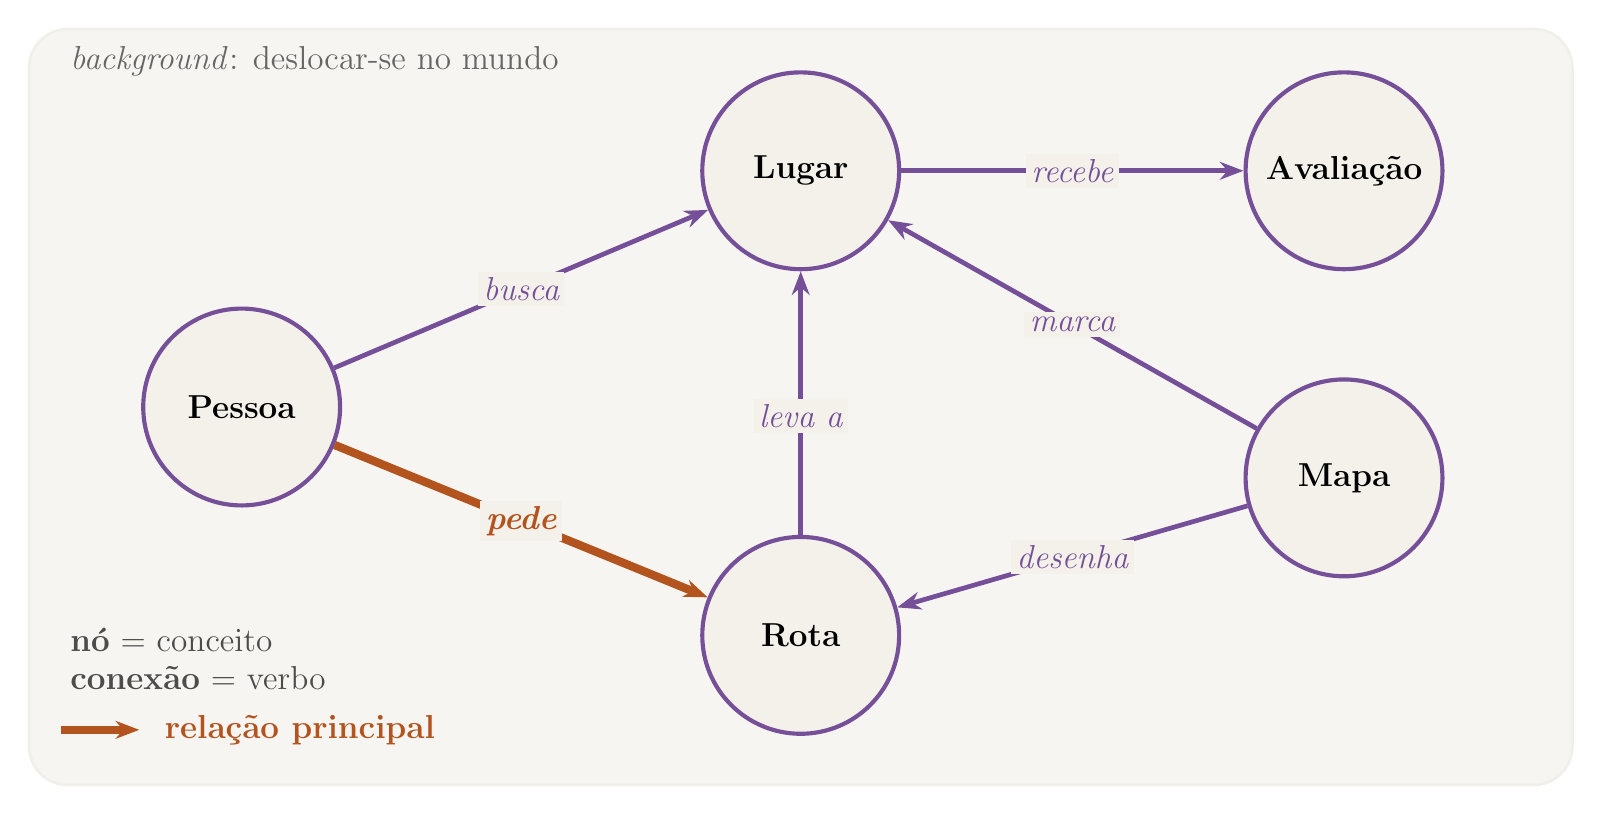
\begin{tikzpicture}[x=1cm,y=1cm]
\tikzset{n/.style={dstate, minimum size=2.5cm, font=\large\bfseries, line width=1.5pt, align=center},
        e/.style={-{Stealth[length=3mm]}, dblue, line width=1.7pt},
        l/.style={midway, fill=dcream, inner sep=2pt, font=\large\itshape}}
\draw[dshade!40, fill=dshade!25, line width=1pt, rounded corners=14pt] (-0.4,-0.6) rectangle (19.2,9.0);
\node[font=\large, black!60, anchor=north west] at (0.0,8.9) {\emph{background}: deslocar-se no mundo};
\node[n, draw=dblue] (p) at (2.3,4.2) {Pessoa};
\node[n, draw=dblue] (g) at (9.4,7.2) {Lugar};
\node[n, draw=dblue] (r) at (9.4,1.3) {Rota};
\node[n, draw=dblue] (m) at (16.3,3.3) {Mapa};
\node[n, draw=dblue] (a) at (16.3,7.2) {Avaliação};
\draw[e] (p) -- node[l] {busca} (g);
\draw[e, dorange, line width=3pt] (p) -- node[l, text=dorange, font=\large\bfseries\itshape] {pede} (r);
\draw[e] (r) -- node[l,pos=0.45] {leva a} (g);
\draw[e] (m) -- node[l] {desenha} (r);
\draw[e] (m) -- node[l] {marca} (g);
\draw[e] (g) -- node[l] {recebe} (a);
\node[font=\large, black!70, align=left, anchor=west] at (0.0,1.0) {\textbf{nó} = conceito\\ \textbf{conexão} = verbo};
\draw[dorange, line width=3pt, -{Stealth[length=3mm]}] (0.0,0.1) -- (1.0,0.1); \node[font=\large\bfseries, dorange, anchor=west] at (1.2,0.1) {relação principal};
\end{tikzpicture}
\end{document}
